\documentclass{article}\usepackage[]{graphicx}\usepackage[]{xcolor}
% maxwidth is the original width if it is less than linewidth
% otherwise use linewidth (to make sure the graphics do not exceed the margin)
\makeatletter
\def\maxwidth{ %
  \ifdim\Gin@nat@width>\linewidth
    \linewidth
  \else
    \Gin@nat@width
  \fi
}
\makeatother

\definecolor{fgcolor}{rgb}{0.345, 0.345, 0.345}
\newcommand{\hlnum}[1]{\textcolor[rgb]{0.686,0.059,0.569}{#1}}%
\newcommand{\hlsng}[1]{\textcolor[rgb]{0.192,0.494,0.8}{#1}}%
\newcommand{\hlcom}[1]{\textcolor[rgb]{0.678,0.584,0.686}{\textit{#1}}}%
\newcommand{\hlopt}[1]{\textcolor[rgb]{0,0,0}{#1}}%
\newcommand{\hldef}[1]{\textcolor[rgb]{0.345,0.345,0.345}{#1}}%
\newcommand{\hlkwa}[1]{\textcolor[rgb]{0.161,0.373,0.58}{\textbf{#1}}}%
\newcommand{\hlkwb}[1]{\textcolor[rgb]{0.69,0.353,0.396}{#1}}%
\newcommand{\hlkwc}[1]{\textcolor[rgb]{0.333,0.667,0.333}{#1}}%
\newcommand{\hlkwd}[1]{\textcolor[rgb]{0.737,0.353,0.396}{\textbf{#1}}}%
\let\hlipl\hlkwb

\usepackage{framed}
\makeatletter
\newenvironment{kframe}{%
 \def\at@end@of@kframe{}%
 \ifinner\ifhmode%
  \def\at@end@of@kframe{\end{minipage}}%
  \begin{minipage}{\columnwidth}%
 \fi\fi%
 \def\FrameCommand##1{\hskip\@totalleftmargin \hskip-\fboxsep
 \colorbox{shadecolor}{##1}\hskip-\fboxsep
     % There is no \\@totalrightmargin, so:
     \hskip-\linewidth \hskip-\@totalleftmargin \hskip\columnwidth}%
 \MakeFramed {\advance\hsize-\width
   \@totalleftmargin\z@ \linewidth\hsize
   \@setminipage}}%
 {\par\unskip\endMakeFramed%
 \at@end@of@kframe}
\makeatother

\definecolor{shadecolor}{rgb}{.97, .97, .97}
\definecolor{messagecolor}{rgb}{0, 0, 0}
\definecolor{warningcolor}{rgb}{1, 0, 1}
\definecolor{errorcolor}{rgb}{1, 0, 0}
\newenvironment{knitrout}{}{} % an empty environment to be redefined in TeX

\usepackage{alltt}
\usepackage{amsmath} %This allows me to use the align functionality.
                     %If you find yourself trying to replicate
                     %something you found online, ensure you're
                     %loading the necessary packages!
\usepackage{amsfonts}%Math font
\usepackage{graphicx}%For including graphics
\usepackage{hyperref}%For Hyperlinks
\usepackage[shortlabels]{enumitem}% For enumerated lists with labels specified
                                  % We had to run tlmgr_install("enumitem") in R
\hypersetup{colorlinks = true,citecolor=black} %set citations to have black (not green) color
\usepackage{natbib}        %For the bibliography
\setlength{\bibsep}{0pt plus 0.3ex}
\bibliographystyle{apalike}%For the bibliography
\usepackage[margin=0.50in]{geometry}
\usepackage{float}
\usepackage{multicol}

%fix for figures
\usepackage{caption}
\newenvironment{Figure}
  {\par\medskip\noindent\minipage{\linewidth}}
  {\endminipage\par\medskip}
\IfFileExists{upquote.sty}{\usepackage{upquote}}{}
\begin{document}

\vspace{-1in}
\title{Lab 02 -- MATH 240 -- Computational Statistics}

\author{
  Jack Schaeffer \\
  Professor Cipolli \\
  MATH 240 \\
  {\tt jschaeffer@colgate.edu}
}

\date{}

\maketitle

\begin{multicols}{2}
\begin{abstract}
This lab focused on using \texttt{R} code to procure data about various songs for analysis. Additionally, the lab focused on skills producing plots and tables to assist with interpretation.
\end{abstract}

\noindent \textbf{Keywords:} Lists; Objects in R, Coding Structures, Graphs, Tables

\section{Introduction}
This lab is focused on the song Allentown, a song released by The Front Bottoms and Manchester Orchestra (and also with additional writing credit to All Get Out). The main question of the lab is determining which artist had the greatest influence on Allentown. To do so, several data processing tools were used. These include Essentia for song analysis and a language analysis tool called LIWC, which utilized JSONLite to manipulate the data in \texttt{R} \citep{essentia} \citep{jsonlite}.

This lab stems from determining what qualities or data about music makes up the total sound,specifically posed by the question of what artist had the greatest influence on the song Allentown. To do so, Essentia can be used to process the data from the songs and determine the characteristics of each individual song \citep{essentia}. Our goal so far through lab has been to prepare executable lines of code that will produce expansive information on each song. Next, this information can be cleaned to prepare for isolating Allentown and comparing it to other songs to determine what artist had the most influence.


\section{Methods}
The brunt of the work done to prepare each song into an executable line of code was handled using various functions in the \texttt{stringr} package to manipulate character names of the file for our desired result \citep{stringr}. To make sure this was done accurately for ever track within a set of given music, two separate for loops were required. \texttt{stringr} was used to determine what folders in a given directory correspond to music albums, and within each song of the album various usage of \texttt{stringr} functions allowed names to be combined for our desired result. Once this manipulation was complete, each iteration ended with the executable line being appended onto a vector that contained each completed line of code.

\subsection{Week 2}
Our goals for week 2 consisted of an introduction in acquiring specific pieces from a list in \texttt{R}. A JSON file was loaded into \texttt{R} using \texttt{jsonlite}, and various objects were created to correspond to the average loudness, key, mean of spectral energy, danceability, bpm, key scale, and length \citep{jsonlite}. Using a dataframe, this information can all be compiled together for each song in an easy to read format. Form here, additional data was collected for each song. Essentia models were sifted to collect additional information on the differing mood values of each song. Finally, additional data was added to the dataframe that included analysis on the lyrics of each song. Once every song properly contained the information, we had a singular dataframe with every song containing the desired characteristics of the music. Finally, separate \texttt{.csv} files were made. In one file we included only the information for Allentown, and in the other file we included every other song. 

\section{Results}
The results of this lab bring us very close to our desired goal of analyzing Allentown to determine what artist had the greater influence on the song. In our initial data compilation during week one, the acquired command lines made it easier to collect information on each song. Now, we have all of the information that is required for each song that will allow insight into Allentown specifically. Now that the information has been successfully pulled together into the dataframe, there is data on the technical construction of the music, the atmosphere or mood each song exhibits, and both technical and practical information considering the lyrical construction. Looking forward for completing the future tasks on this lab, the data will be analyzed in order to come to conclusions on Allentown's composition and other insight that can be gained from the data we collected this week.

\begin{figure}[H]
 \begin{center}
 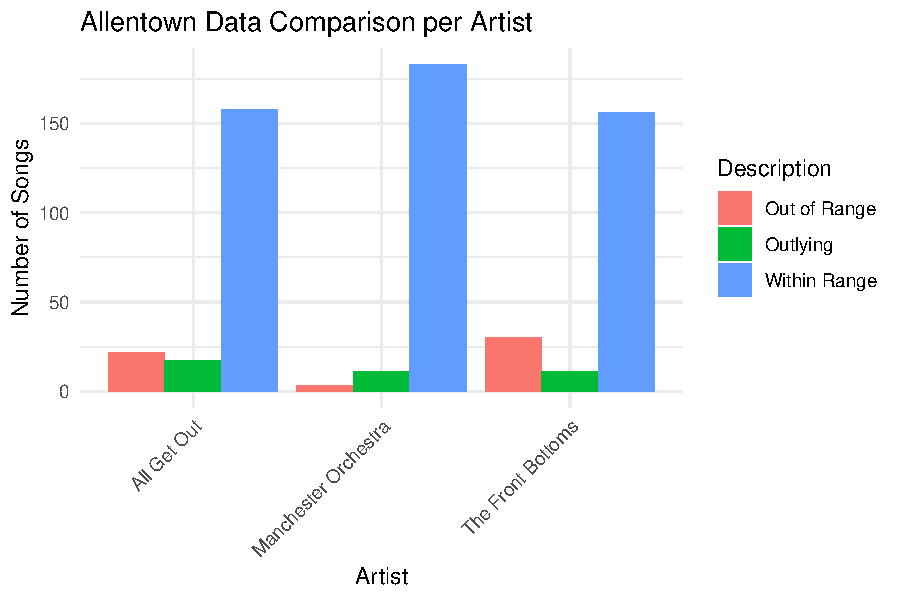
\includegraphics[scale=0.65]{descript_plot.pdf}
 \caption{A comparison of Allentown's data to each artist}
 \label{plot3}
 \end{center}
 \end{figure}






% latex table generated in R 4.4.2 by xtable 1.8-4 package
% Tue Feb 25 11:57:26 2025
\begin{table}[H]
\centering
\begingroup\small
\begin{tabular}{llr}
  \hline
Artist & Description & Count \\ 
  \hline
All Get Out & Out of Range &  22 \\ 
  All Get Out & Outlying &  17 \\ 
  All Get Out & Within Range & 158 \\ 
  Manchester Orchestra & Out of Range &   3 \\ 
  Manchester Orchestra & Outlying &  11 \\ 
  Manchester Orchestra & Within Range & 183 \\ 
  The Front Bottoms & Out of Range &  30 \\ 
  The Front Bottoms & Outlying &  11 \\ 
  The Front Bottoms & Within Range & 156 \\ 
   \hline
\end{tabular}
\endgroup
\label{count.tab}
\end{table}






%%%%%%%%%%%%%%%%%%%%%%%%%%%%%%%%%%%%%%%%%%%%%%%%%%%%%%%%%%%%%%%%%%%%%%%%%%%%%%%%
% Bibliography
%%%%%%%%%%%%%%%%%%%%%%%%%%%%%%%%%%%%%%%%%%%%%%%%%%%%%%%%%%%%%%%%%%%%%%%%%%%%%%%%
\vspace{2em}

\noindent\textbf{Bibliography:} Note that when you add citations to your bib.bib file \emph{and}
you cite them in your document, the bibliography section will automatically populate here.

\begin{tiny}
\bibliography{bib}
\end{tiny}
\end{multicols}

%%%%%%%%%%%%%%%%%%%%%%%%%%%%%%%%%%%%%%%%%%%%%%%%%%%%%%%%%%%%%%%%%%%%%%%%%%%%%%%%
% Appendix
%%%%%%%%%%%%%%%%%%%%%%%%%%%%%%%%%%%%%%%%%%%%%%%%%%%%%%%%%%%%%%%%%%%%%%%%%%%%%%%%


\end{document}
